\section{Reproducibility Checklist}
\seclabel{appendix:checklist}
\subsection{Computing infrastructure}
We use four Tesla V100 GPUs to prompt
each of the \mdrs, and
a single Tesla V100 GPU
is used when finetuning the small model
$\mathcal{S}$.

\subsection{Datasets}
For SST2, CoLA, and RTE, we use the official datasets
available on the benchmark website
\url{gluebenchmark.com}.
We download
SST5 dataset from
\url{nlp.stanford.edu/sentiment}
and AGNews
from the link provided by \citet{agdataset}.

The number of testing examples of each dataset
is shown in \tabref{appendix:numtestegs}.
Note that for SST2, CoLA, and RTE,
$\mathcal{G}^{dev}$ is sampled from
the training set, and the dev set is used as the test set.

\begin{table}[h]
\small\centering
\begin{tabular}{|c|c|c|c|c|}
\hline
CoLA & SST5 & RTE & AGNews & SST2 \\ \hline
1042 & 2210 & 277 & 7600   & 872  \\ \hline
\end{tabular}
\caption{Number of testing examples.}
\tablabel{appendix:numtestegs}
\end{table}

\begin{table*}[h]
\centering\scriptsize\renewcommand{\arraystretch}{1.2}\setlength{\tabcolsep}{4pt}
\begin{tabular}{c|cc|cc|cc|}
\cline{2-7}
                             & \multicolumn{2}{c|}{$\mathcal{G}^8$}                    & \multicolumn{2}{c|}{$\mathcal{G}^{16}$}                 & \multicolumn{2}{c|}{$\mathcal{G}^{32}$}                    \\ \cline{2-7} 
                             & \multicolumn{1}{c|}{Workers}        &  $\mathcal{S}$    & \multicolumn{1}{c|}{Workers}        & $\mathcal{S}$     & \multicolumn{1}{c|}{Workers}        & $\mathcal{S}$             \\ \hline
\multicolumn{1}{|c|}{}       & \multicolumn{1}{c|}{91.13$\pm$0.52} &                   & \multicolumn{1}{c|}{91.93$\pm$1.09} &                   & \multicolumn{1}{c|}{91.97$\pm$0.83} &                   \\
\multicolumn{1}{|c|}{}       & \multicolumn{1}{c|}{91.63$\pm$0.68} &                   & \multicolumn{1}{c|}{93.08$\pm$0.62} &                   & \multicolumn{1}{c|}{91.70$\pm$1.78} &                   \\
\multicolumn{1}{|c|}{SST2}   & \multicolumn{1}{c|}{90.18$\pm$1.00} & 67.63$\pm$8.01    & \multicolumn{1}{c|}{91.74$\pm$1.04} & 75.83$\pm$1.35    & \multicolumn{1}{c|}{91.21$\pm$1.83} & 76.37$\pm$3.16 \\
\multicolumn{1}{|c|}{}       & \multicolumn{1}{c|}{90.83$\pm$0.58} &                   & \multicolumn{1}{c|}{90.79$\pm$0.47} &                   & \multicolumn{1}{c|}{91.13$\pm$0.24} &                   \\
\multicolumn{1}{|c|}{}       & \multicolumn{1}{c|}{90.52$\pm$1.84} &                   & \multicolumn{1}{c|}{91.67$\pm$1.36} &                   & \multicolumn{1}{c|}{93.23$\pm$0.37} &                   \\ \hline
\multicolumn{1}{|c|}{}       & \multicolumn{1}{c|}{41.37$\pm$1.55} &                   & \multicolumn{1}{c|}{45.16$\pm$2.13} &                   & \multicolumn{1}{c|}{45.91$\pm$0.96} &                   \\
\multicolumn{1}{|c|}{}       & \multicolumn{1}{c|}{42.32$\pm$2.04} &                   & \multicolumn{1}{c|}{45.96$\pm$2.12} &                   & \multicolumn{1}{c|}{48.64$\pm$0.59} &                   \\
\multicolumn{1}{|c|}{SST5}   & \multicolumn{1}{c|}{40.57$\pm$2.70} & 28.47$\pm$1.61    & \multicolumn{1}{c|}{46.70$\pm$0.93} & 34.97$\pm$1.51    & \multicolumn{1}{c|}{50.53$\pm$0.94} & 33.47$\pm$2.79 \\
\multicolumn{1}{|c|}{}       & \multicolumn{1}{c|}{37.69$\pm$1.34} &                   & \multicolumn{1}{c|}{42.53$\pm$2.43} &                   & \multicolumn{1}{c|}{43.32$\pm$3.42} &                   \\
\multicolumn{1}{|c|}{}       & \multicolumn{1}{c|}{38.05$\pm$2.60} &                   & \multicolumn{1}{c|}{42.96$\pm$0.69} &                   & \multicolumn{1}{c|}{45.72$\pm$1.43} &                   \\ \hline
\multicolumn{1}{|c|}{}       & \multicolumn{1}{c|}{68.95$\pm$1.47} &                   & \multicolumn{1}{c|}{68.35$\pm$2.29} &                   & \multicolumn{1}{c|}{71.72$\pm$1.96} &                   \\
\multicolumn{1}{|c|}{}       & \multicolumn{1}{c|}{54.99$\pm$3.76} &                   & \multicolumn{1}{c|}{57.64$\pm$3.23} &                   & \multicolumn{1}{c|}{58.48$\pm$3.59} &                   \\
\multicolumn{1}{|c|}{RTE}    & \multicolumn{1}{c|}{62.70$\pm$1.33} & 57.30$\pm$1.79    & \multicolumn{1}{c|}{70.88$\pm$1.70} & 61.50$\pm$0.78    & \multicolumn{1}{c|}{68.47$\pm$1.19} & 62.93$\pm$0.74 \\
\multicolumn{1}{|c|}{}       & \multicolumn{1}{c|}{50.42$\pm$2.07} &                   & \multicolumn{1}{c|}{58.60$\pm$1.62} &                   & \multicolumn{1}{c|}{59.33$\pm$4.72} &                   \\
\multicolumn{1}{|c|}{}       & \multicolumn{1}{c|}{51.99$\pm$4.45} &                   & \multicolumn{1}{c|}{57.88$\pm$2.83} &                   & \multicolumn{1}{c|}{60.41$\pm$2.47} &                   \\ \hline
\multicolumn{1}{|c|}{}       & \multicolumn{1}{c|}{75.39$\pm$5.25} &                   & \multicolumn{1}{c|}{83.06$\pm$0.83} &                   & \multicolumn{1}{c|}{84.92$\pm$0.28} &                   \\
\multicolumn{1}{|c|}{}       & \multicolumn{1}{c|}{85.40$\pm$1.43} &                   & \multicolumn{1}{c|}{87.71$\pm$0.07} &                   & \multicolumn{1}{c|}{87.79$\pm$1.08} &                   \\
\multicolumn{1}{|c|}{AGNews} & \multicolumn{1}{c|}{78.83$\pm$4.77} & 66.37$\pm$2.95    & \multicolumn{1}{c|}{83.59$\pm$2.96} & 69.40$\pm$0.93    & \multicolumn{1}{c|}{87.39$\pm$1.29} & 76.53$\pm$0.41 \\
\multicolumn{1}{|c|}{}       & \multicolumn{1}{c|}{85.07$\pm$1.09} &                   & \multicolumn{1}{c|}{87.69$\pm$0.04} &                   & \multicolumn{1}{c|}{87.17$\pm$0.67} &                   \\
\multicolumn{1}{|c|}{}       & \multicolumn{1}{c|}{79.95$\pm$0.86} &                   & \multicolumn{1}{c|}{80.15$\pm$3.38} &                   & \multicolumn{1}{c|}{83.32$\pm$0.59} &                   \\ \hline
\multicolumn{1}{|c|}{}       & \multicolumn{1}{c|}{ 0.14$\pm$1.43} &                   & \multicolumn{1}{c|}{11.81$\pm$7.82} &                   & \multicolumn{1}{c|}{19.88$\pm$3.30} &                   \\
\multicolumn{1}{|c|}{}       & \multicolumn{1}{c|}{ 2.42$\pm$4.84} &                   & \multicolumn{1}{c|}{15.23$\pm$7.07} &                   & \multicolumn{1}{c|}{22.51$\pm$0.96} &                   \\
\multicolumn{1}{|c|}{CoLA}   & \multicolumn{1}{c|}{ 7.40$\pm$8.12} & 0.97$\pm$4.40     & \multicolumn{1}{c|}{19.71$\pm$1.89} & 4.27$\pm$3.26     & \multicolumn{1}{c|}{26.34$\pm$1.54} & 2.50$\pm$2.41 \\
\multicolumn{1}{|c|}{}       & \multicolumn{1}{c|}{ 9.91$\pm$7.98} &                   & \multicolumn{1}{c|}{17.14$\pm$2.48} &                   & \multicolumn{1}{c|}{18.15$\pm$0.63} &                   \\
\multicolumn{1}{|c|}{}       & \multicolumn{1}{c|}{15.33$\pm$2.15} &                   & \multicolumn{1}{c|}{19.66$\pm$0.48} &                   & \multicolumn{1}{c|}{27.58$\pm$7.09} &                   \\ \hline
\end{tabular}
\caption{Few-shot performance of the five \mdrs
  and the small model $\mathcal{S}$.
  Each experiment is repeated three times and we report mean and standard deviation.}
\tablabel{appendix:fewshotnumeric}
\end{table*}


%%% Local Variables:
%%% mode: latex
%%% TeX-master: "acl_latex"
%%% End:


\section{Numerical Results}
\seclabel{appendix:numeric}
\tabref{appendix:fewshotnumeric}
reports the numerical
value of \figref{fewshotperf}.


\section{Prompting Details}
\seclabel{appendix:promptingdetails}
For each task, 
we list the five prompts
employed to adapt a PLM  to a \mdr.
``[v]'' is a prompting token whose
trainable embedding vector is 
randomly initialized.

For \textbf{SST5}, we use following prompts:
\begin{itemize}
\item ``[v] \textbf{x} It is [MASK].''
\item ``[v] \textbf{x} Such a [MASK] movie.''
\item ``\textbf{x} [v] It is pretty [MASK].''
\item ``It is [MASK] because \textbf{x} [v]''
\item ``\textbf{x} So it is [MASK]. [v]''
\end{itemize}
and the PLM picks a word from
\{``crap'', ``bad'', ``normal'', ``good'', ``perfect''\}.
to fill the position of ``[MASK]''.
The mapping
\{``crap''$\,\to\,$1,
``bad''$\,\to\,$2,
``normal''$\,\to\,$3,
``good''$\,\to\,$4,
``perfect''$\,\to\,$5
\} is used to convert
model predictions to numerical values.


For \textbf{SST2}, we use following prompts:
\begin{itemize}
\item ``[v] \textbf{x} It is [MASK].''
\item ``[v] \textbf{x} Such a [MASK] movie.''
\item ``\textbf{x} [v] It is pretty [MASK].''
\item ``It is [MASK] because \textbf{x} [v]''
\item ``\textbf{x} So it is [MASK]. [v]''
\end{itemize}
and the PLM picks a word from
\{``bad'', ``good''\}
to fill the position of ``[MASK]''.
The mapping
\{``bad''$\,\to\,$0, ``good''$\,\to\,$1\}
is used.



For \textbf{AGNews}, we use following prompts:
\begin{itemize}
\item ``[v] \textbf{x} It is about [MASK].''
\item ``\textbf{x} [v] Topic: [MASK].''
\item ``\textbf{x} [v] The text is about [MASK].''
\item ``\textbf{x} Topic: [MASK]. [v]''
\item ``\textbf{x} [v] [MASK].''
\end{itemize}
and the PLM picks a word from
\{``world'', ``sports'', ``economy'', ``technology''\}
to fill the position of ``[MASK]''.
The mapping
\{``world''$\,\to\,$1,
``sports''$\,\to\,$2,
``economy''$\,\to\,$3,
``technology''$\,\to\,$4
\} is used.


For \textbf{CoLA}, we use following prompts:
\begin{itemize}
\item ``[v] \textbf{x} It sounds [MASK].''
\item ``[v] \textbf{x} The sentence is [MASK].''
\item ``[v] \textbf{x} It is a [MASK] sentence.''
\item ``\textbf{x} [v] [MASK].''
\item ``[v] \textbf{x} [MASK].''
\end{itemize}
and the PLM picks a word from
\{``wrong'', ``ok''\}
to fill the position of ``[MASK]''.
The mapping
\{``wrong''$\,\to\,$0,
``okay''$\,\to\,$1\}
is used.


For \textbf{RTE}, we use following prompts:
\begin{itemize}
\item ``\textbf{p} Question: \textbf{h}? [v] Answer: [MASK].''
\item ``\textbf{p} [SEP] \textbf{h}? [MASK]. [v]''
\item ``\textbf{p} [SEP] \textbf{h}? [v] answer: [MASK].''
\item ``\textbf{p} [SEP] In short \textbf{h}. [MASK]. [v]''
\item ``[v] \textbf{p} [SEP] In short \textbf{h}. [MASK].''
\end{itemize}
where \textbf{p} and \textbf{h}
refer to premise and hypothesis.
The PLM picks a word from
\{``No'', ``Yes''\}
to fill the position of ``[MASK]''.
The mapping
\{``No''$\,\to\,$0,
``Yes''$\,\to\,$1\}
is used.

\begin{figure}[t]
\centering
\vspace{-.25cm}\subfloat{
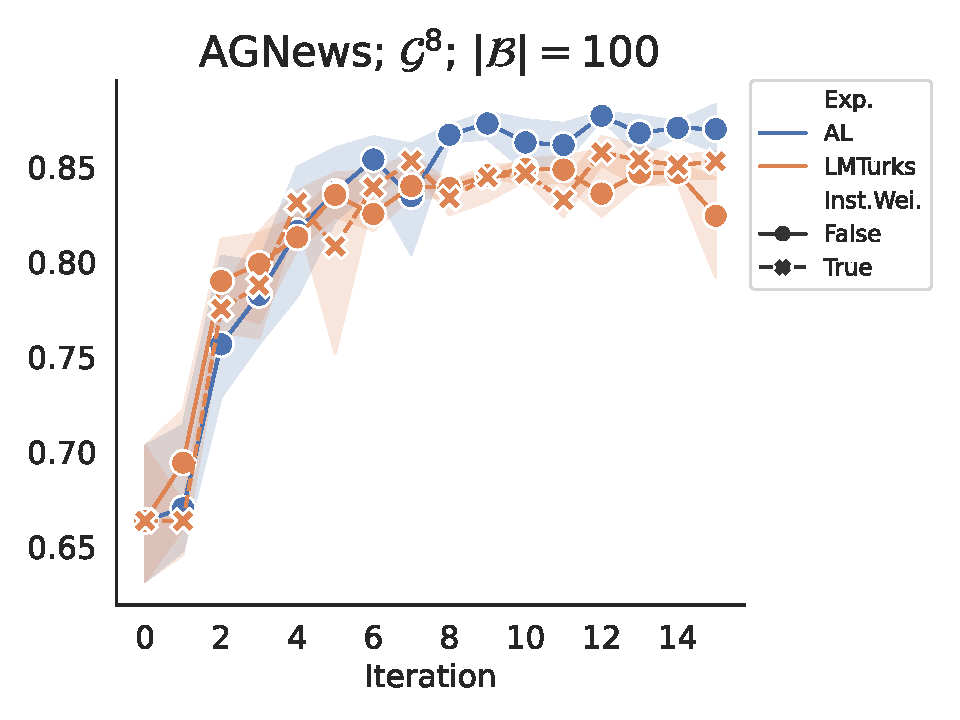
\includegraphics[width=.5\linewidth,height=0.18\textwidth]{imgs/IW,ag,8,100.pdf}
}
\vspace{-.25cm}\subfloat{
\hspace{-.25cm}
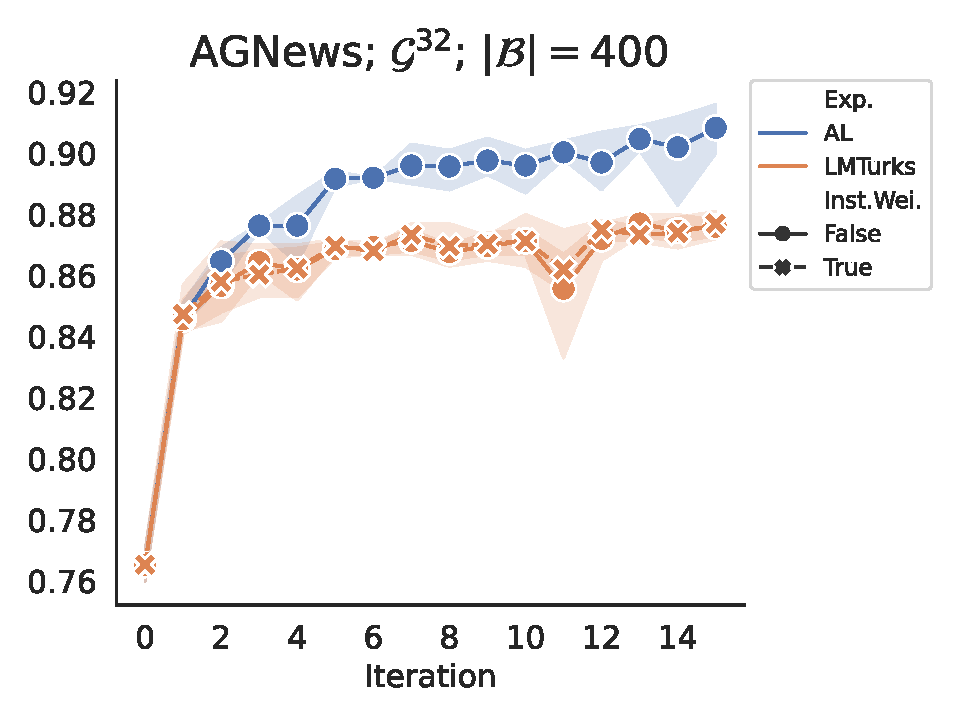
\includegraphics[width=.5\linewidth,height=0.18\textwidth]{imgs/IW,ag,32,400.pdf}
}
\\
\vspace{-.25cm}\subfloat{
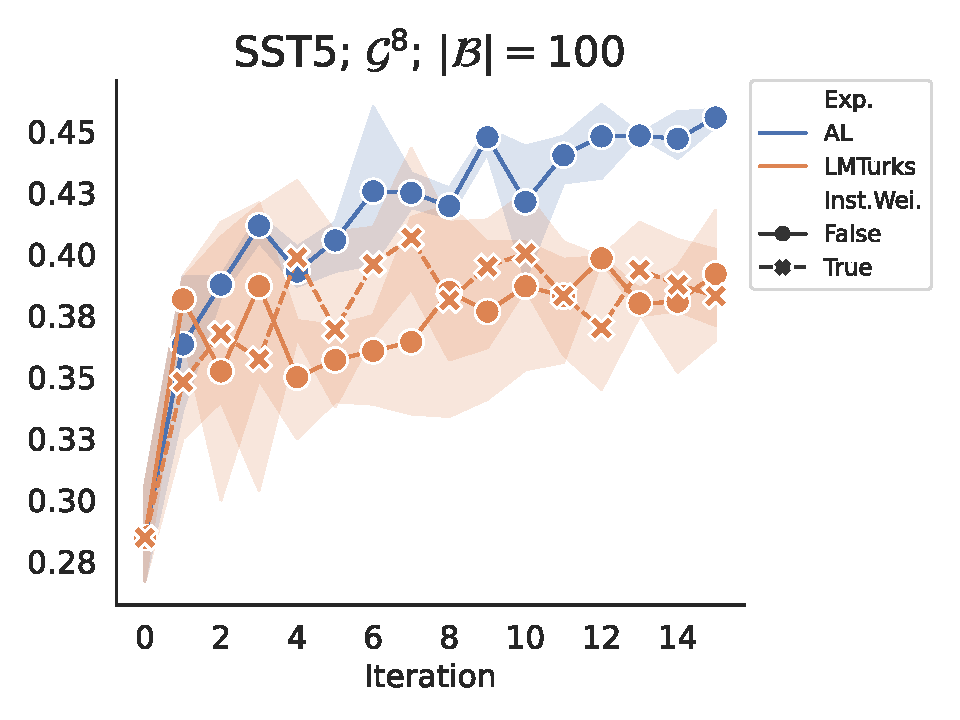
\includegraphics[width=.5\linewidth,height=0.18\textwidth]{imgs/IW,sst5,8,100.pdf}
}
\vspace{-.25cm}\subfloat{
\hspace{-.25cm}    
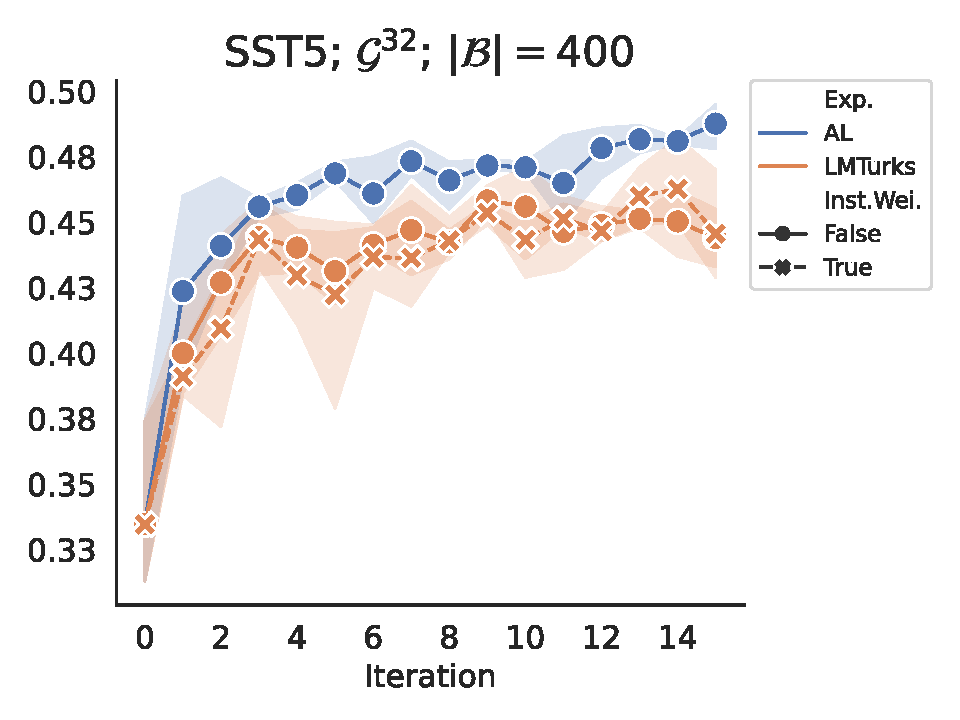
\includegraphics[width=.5\linewidth,height=0.18\textwidth]{imgs/IW,sst5,32,400.pdf}
}
\\
\vspace{-.25cm}\subfloat{
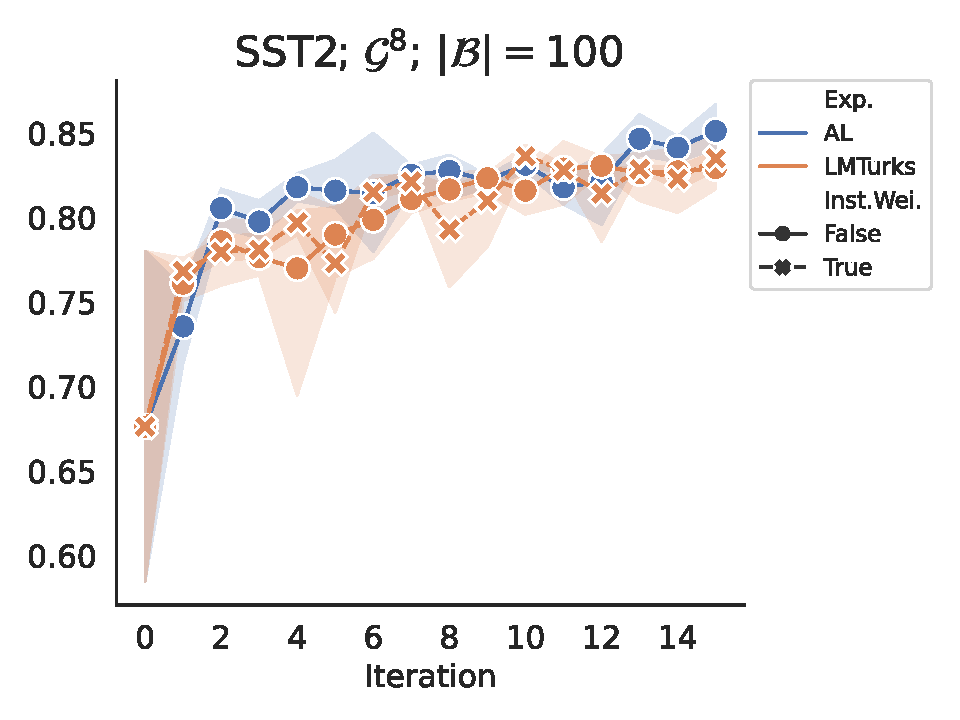
\includegraphics[width=.5\linewidth,height=0.18\textwidth]{imgs/IW,sst2,8,100.pdf}
}
\vspace{-.25cm}\subfloat{
\hspace{-.25cm}  
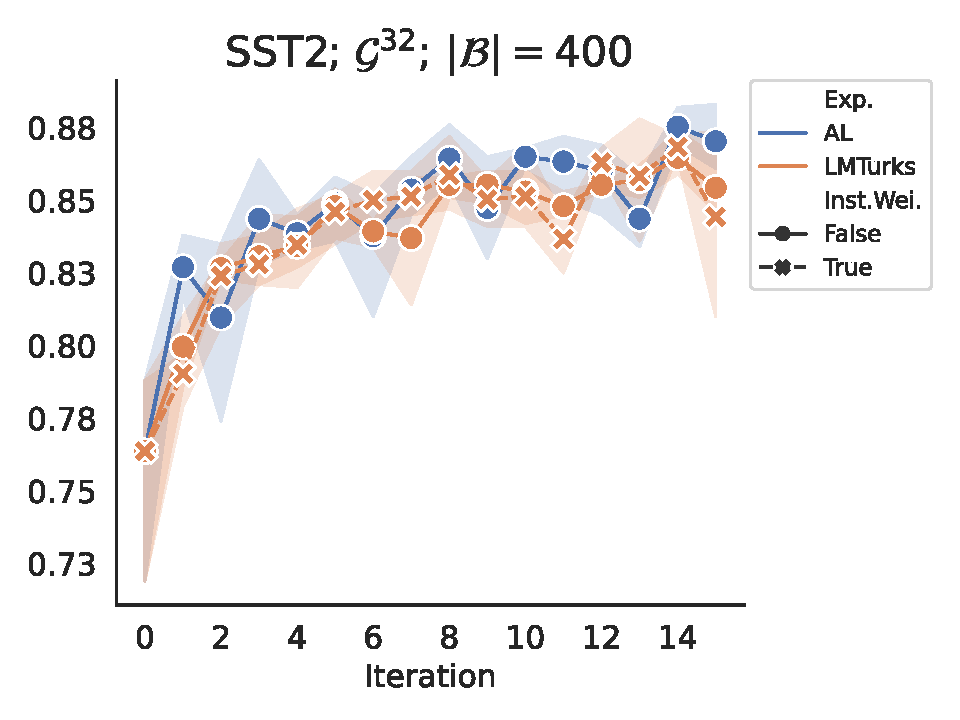
\includegraphics[width=.5\linewidth,height=0.18\textwidth]{imgs/IW,sst2,32,400.pdf}
}
\caption{
Weighting the training instances from \mdrs.
}
\figlabel{instanceweighting}
\end{figure}




\section{More Visualizations}
\seclabel{appendix:morevisualization}
\figref{appendix:completeiteratives} visualizes the performance
of $\mathcal{S}$ when different $|\mathcal{G}|$ and
$|\mathcal{B}|$ are used.


\begin{figure*}[t]
\centering
\hspace{-.2cm}\subfloat{
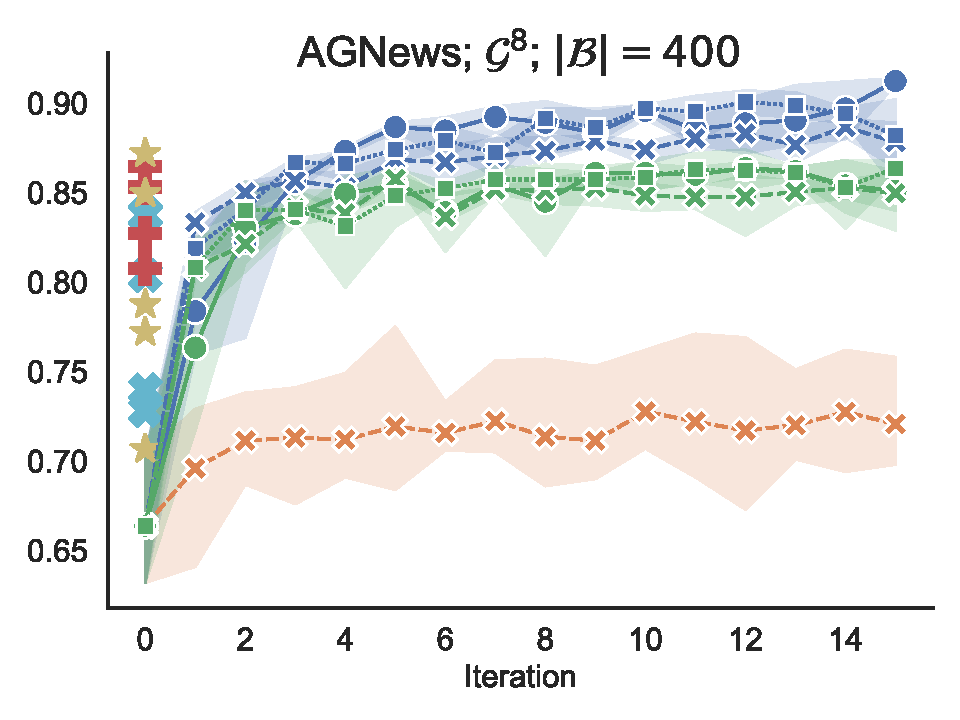
\includegraphics[width=.25\linewidth,height=0.2\textwidth]{imgs/appendix/_ag,MV,8,400.pdf}
}
\hspace{-.2cm}\subfloat{
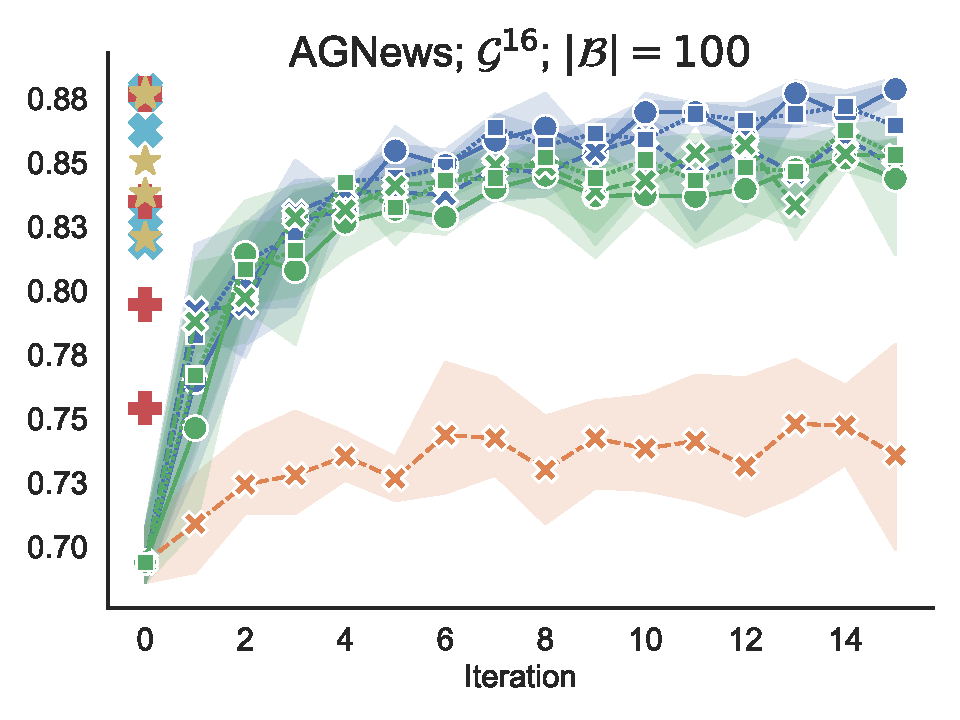
\includegraphics[width=.25\linewidth,height=0.2\textwidth]{imgs/appendix/_ag,MV,16,100.pdf}
}
\hspace{-.2cm}\subfloat{
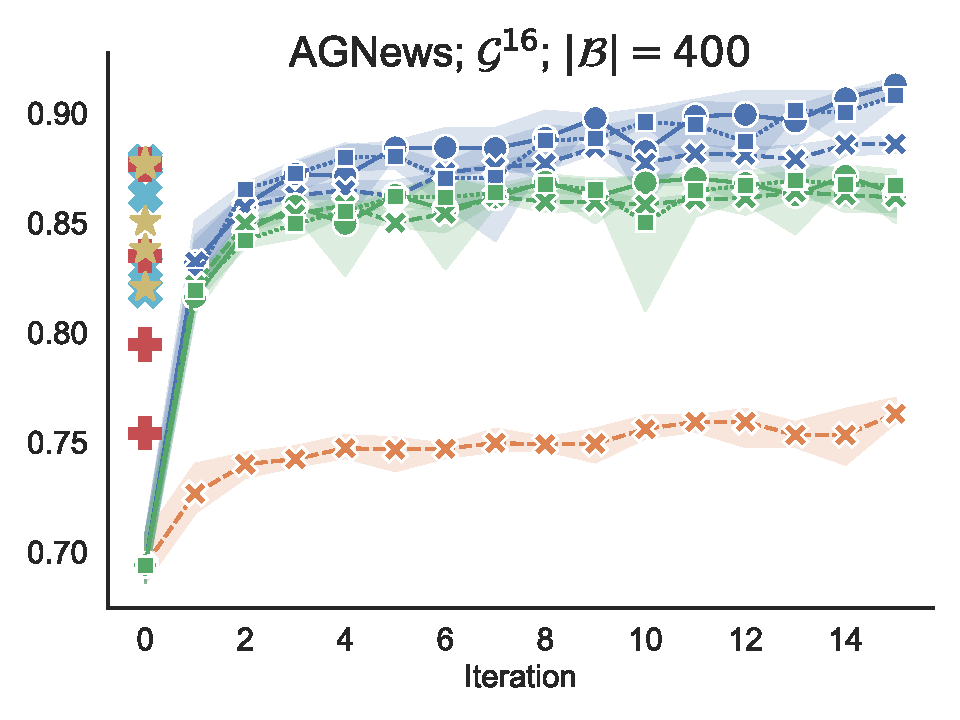
\includegraphics[width=.25\linewidth,height=0.2\textwidth]{imgs/appendix/_ag,MV,16,400.pdf}
}
\hspace{-.2cm}\subfloat{
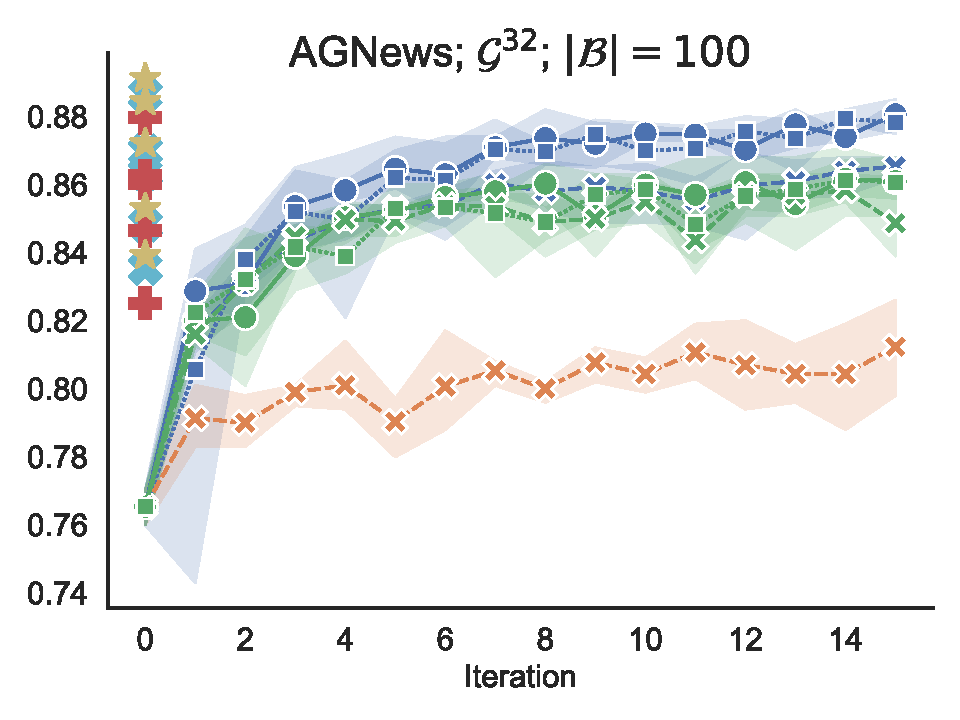
\includegraphics[width=.25\linewidth,height=0.2\textwidth]{imgs/appendix/_ag,MV,32,100.pdf}
}
\\
\hspace{-.2cm}\subfloat{
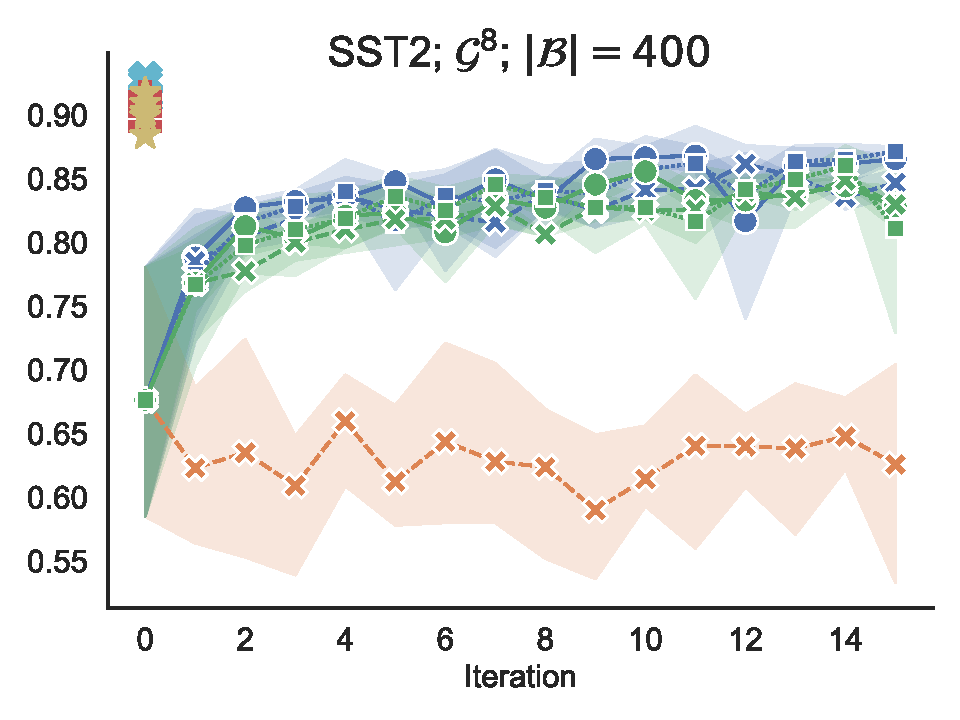
\includegraphics[width=.25\linewidth,height=0.2\textwidth]{imgs/appendix/_sst2,MV,8,400.pdf}
}
\hspace{-.2cm}\subfloat{
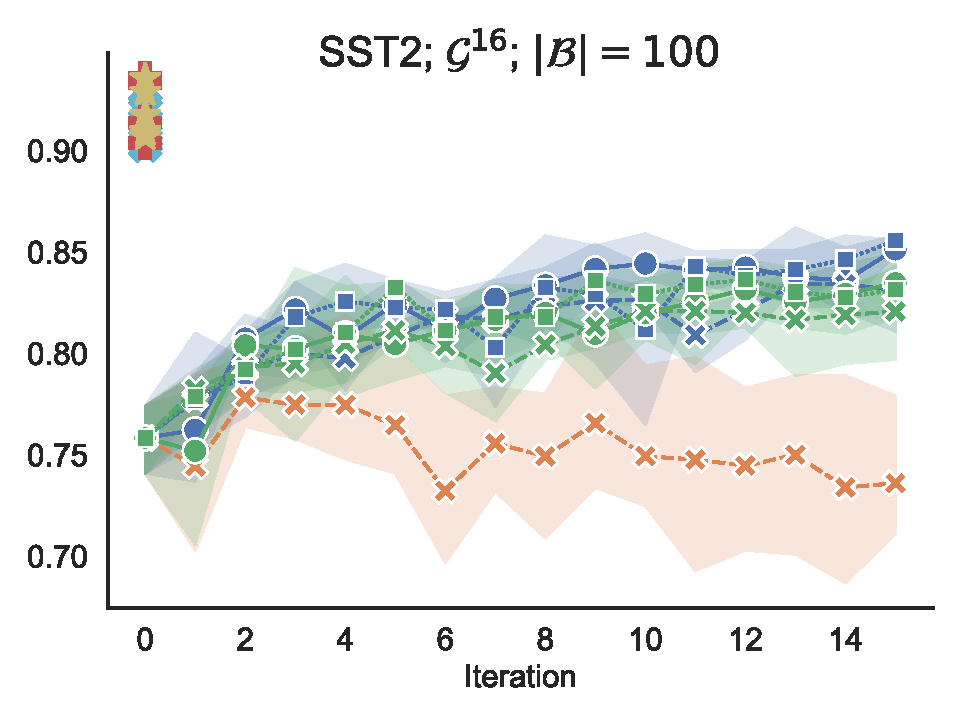
\includegraphics[width=.25\linewidth,height=0.2\textwidth]{imgs/appendix/_sst2,MV,16,100.pdf}
}
\hspace{-.2cm}\subfloat{
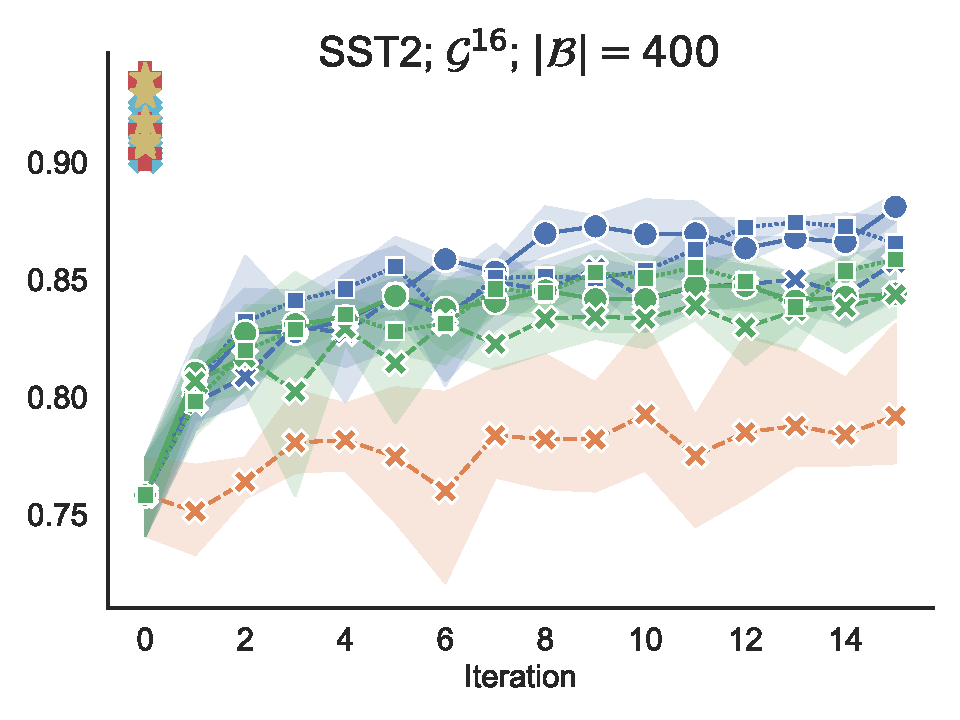
\includegraphics[width=.25\linewidth,height=0.2\textwidth]{imgs/appendix/_sst2,MV,16,400.pdf}
}
\hspace{-.2cm}\subfloat{
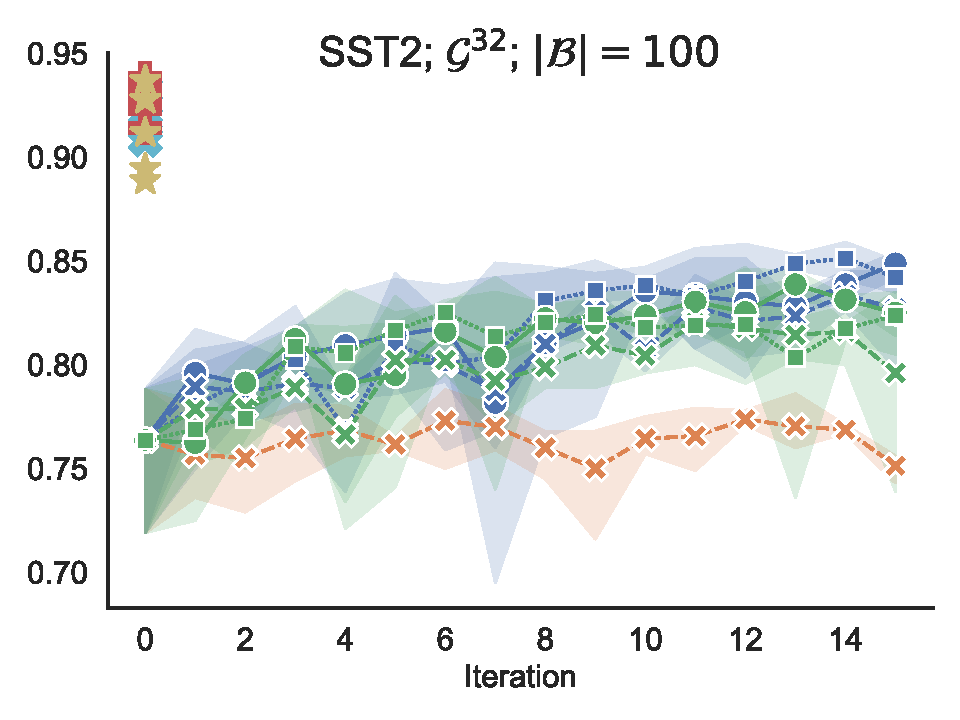
\includegraphics[width=.25\linewidth,height=0.2\textwidth]{imgs/appendix/_sst2,MV,32,100.pdf}
}
\\
\hspace{-.2cm}\subfloat{
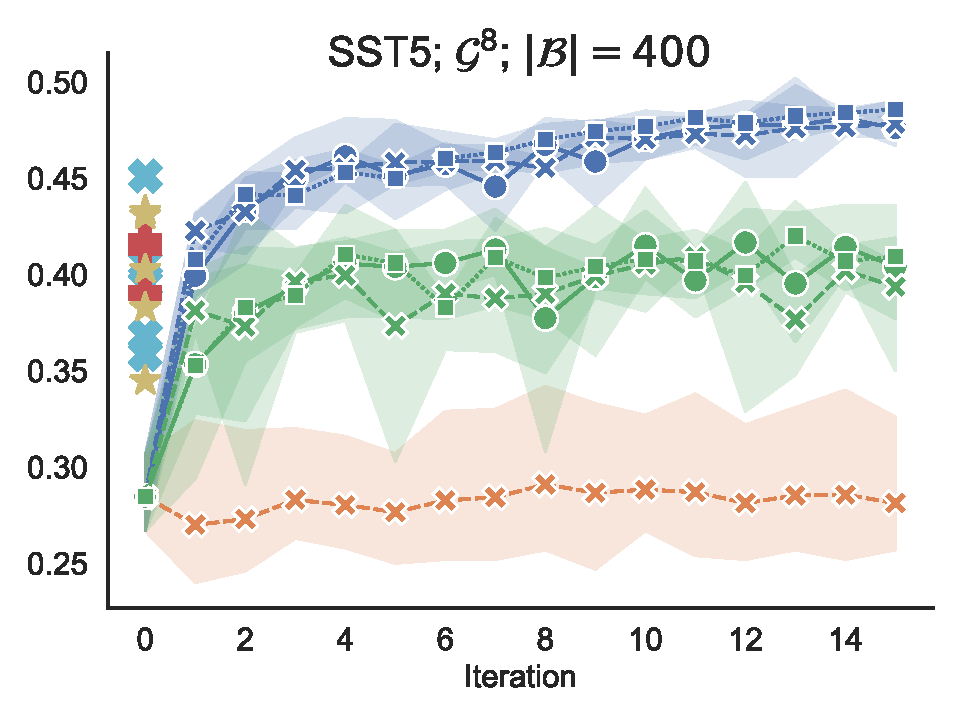
\includegraphics[width=.25\linewidth,height=0.2\textwidth]{imgs/appendix/_sst5,MV,8,400.pdf}
}
\hspace{-.2cm}\subfloat{
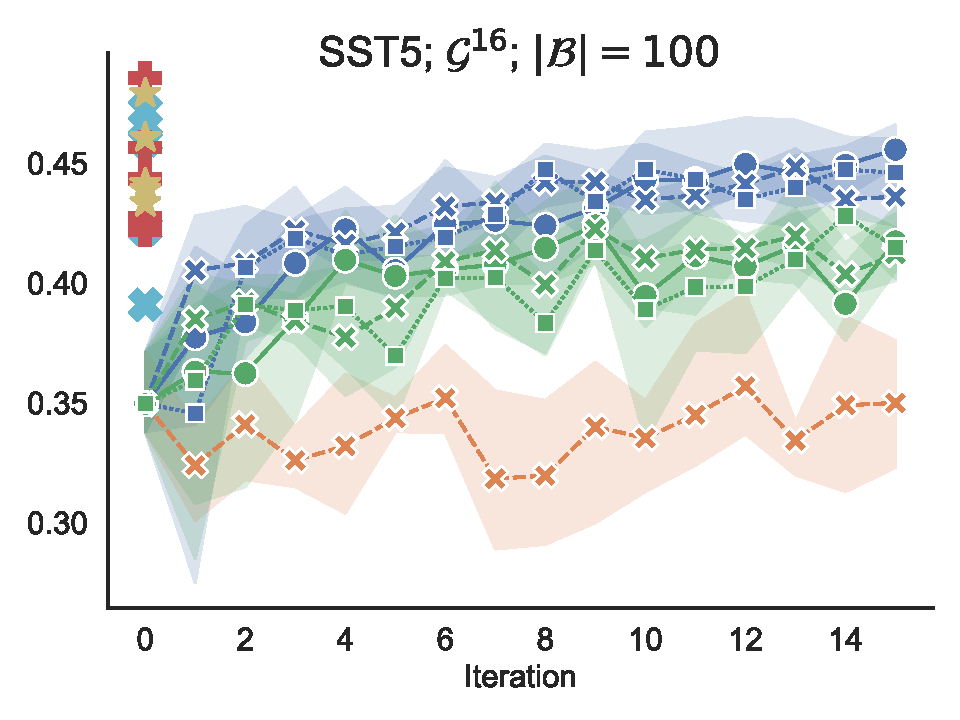
\includegraphics[width=.25\linewidth,height=0.2\textwidth]{imgs/appendix/_sst5,MV,16,100.pdf}
}
\hspace{-.2cm}\subfloat{
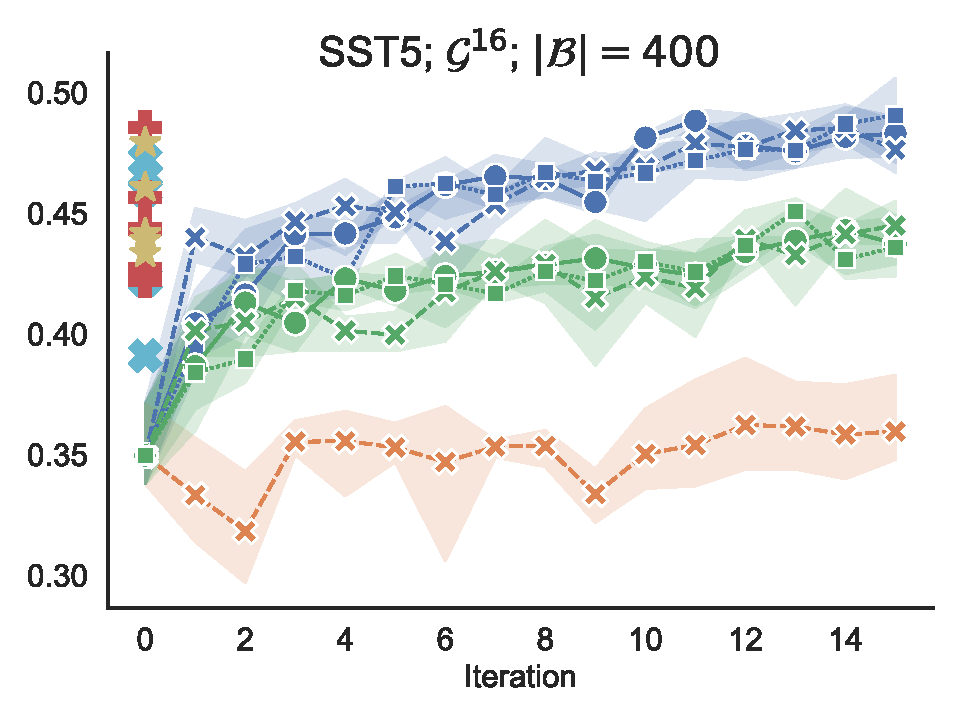
\includegraphics[width=.25\linewidth,height=0.2\textwidth]{imgs/appendix/_sst5,MV,16,400.pdf}
}
\hspace{-.2cm}\subfloat{
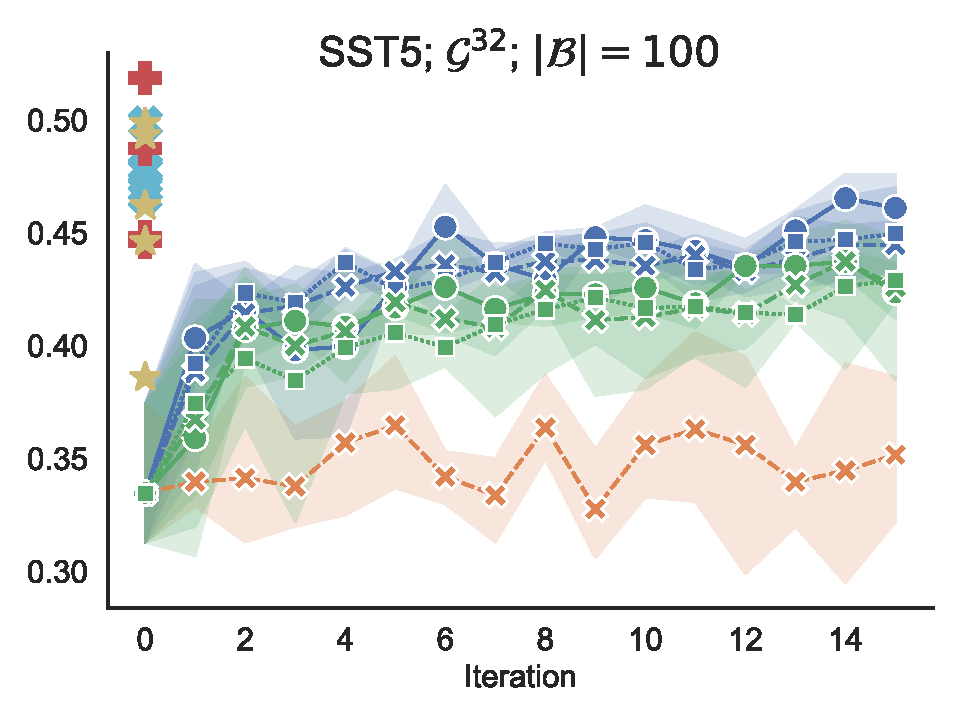
\includegraphics[width=.25\linewidth,height=0.2\textwidth]{imgs/appendix/_sst5,MV,32,100.pdf}
}
\\
\hspace{-.2cm}\subfloat{
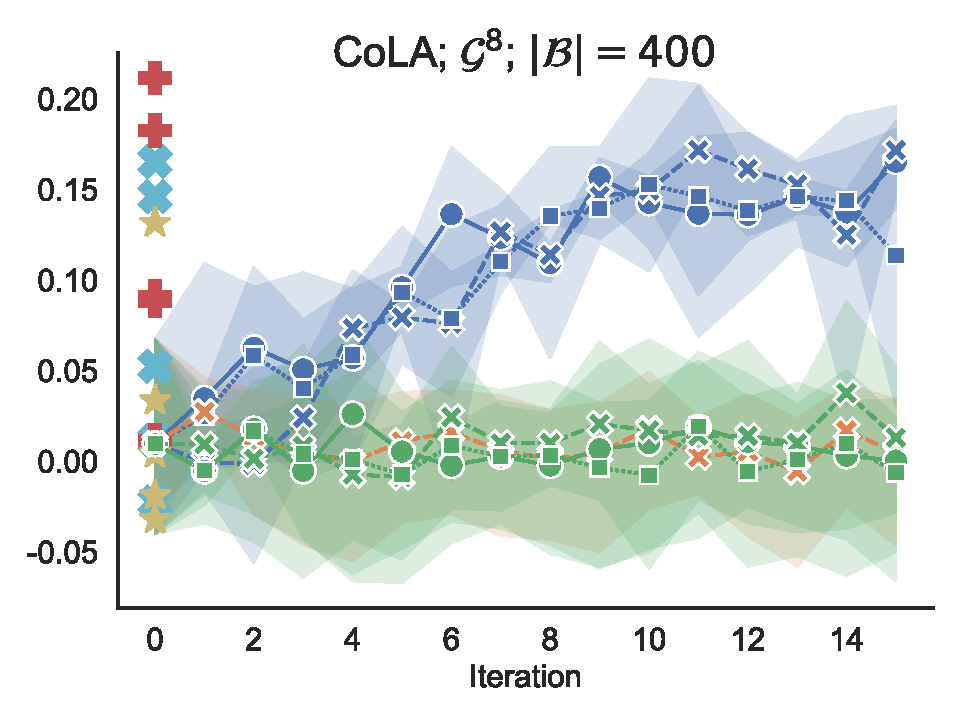
\includegraphics[width=.25\linewidth,height=0.2\textwidth]{imgs/appendix/_cola,MV,8,400.pdf}
}
\hspace{-.2cm}\subfloat{
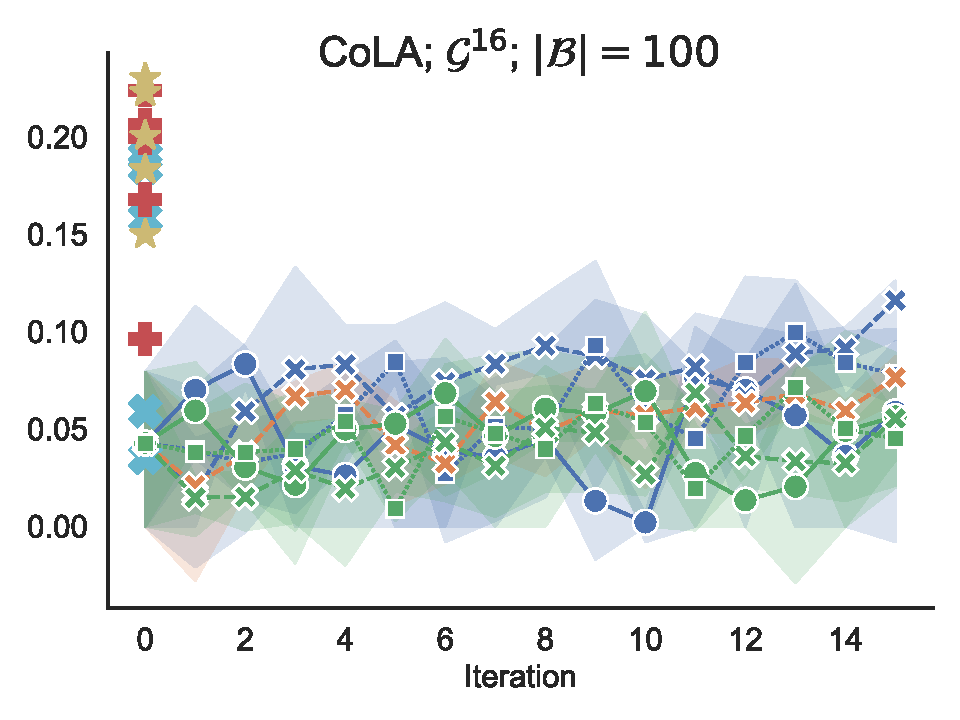
\includegraphics[width=.25\linewidth,height=0.2\textwidth]{imgs/appendix/_cola,MV,16,100.pdf}
}
\hspace{-.2cm}\subfloat{
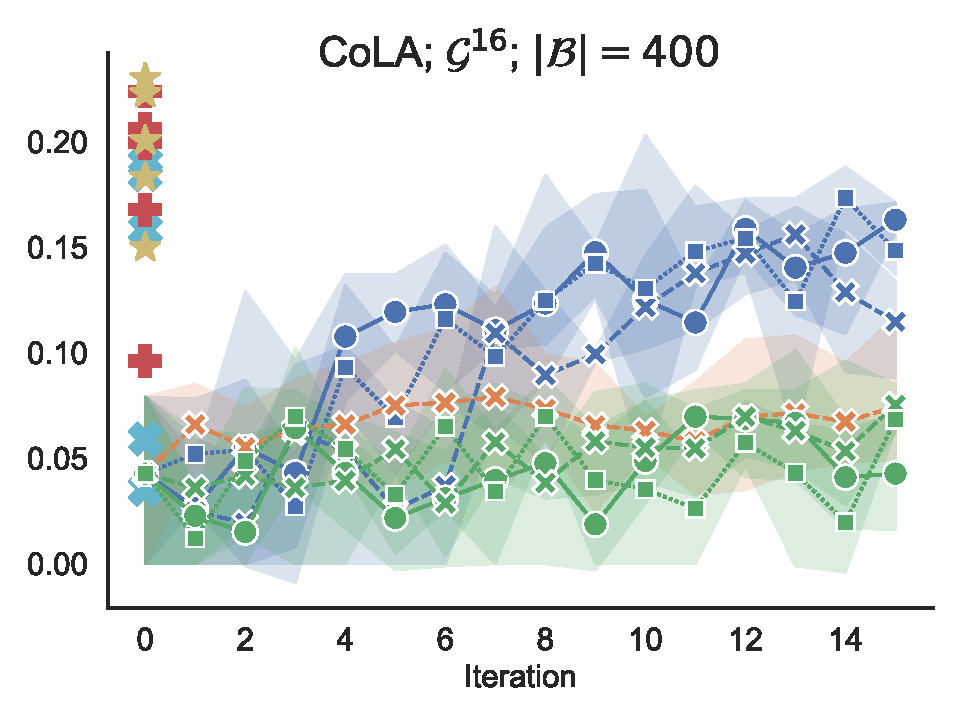
\includegraphics[width=.25\linewidth,height=0.2\textwidth]{imgs/appendix/_cola,MV,16,400.pdf}
}
\hspace{-.2cm}\subfloat{
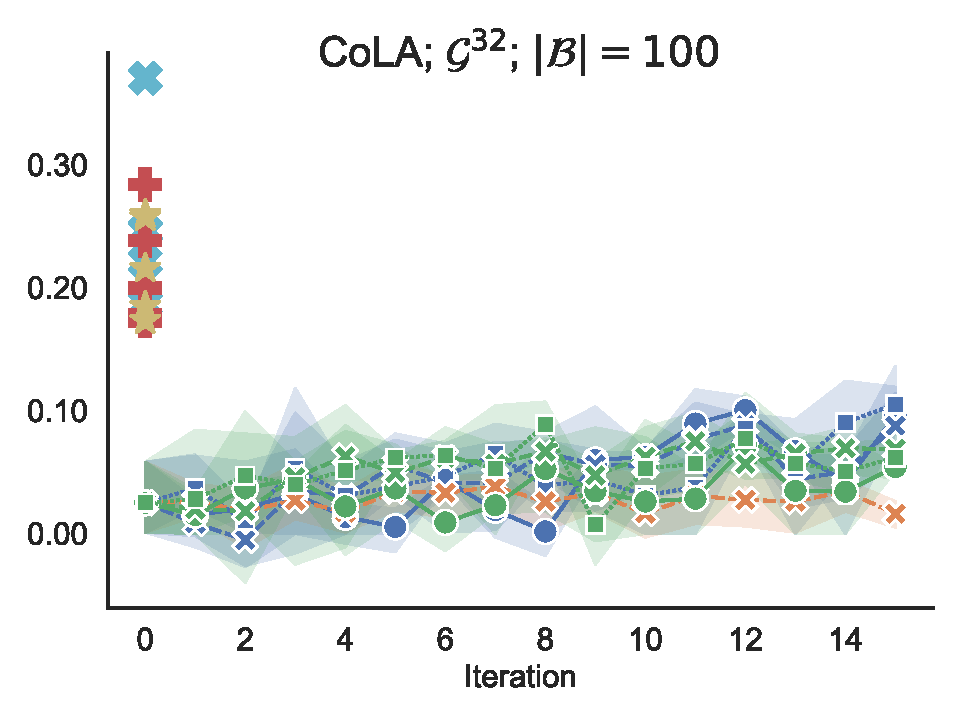
\includegraphics[width=.25\linewidth,height=0.2\textwidth]{imgs/appendix/_cola,MV,32,100.pdf}
}
\\
\hspace{-.2cm}\subfloat{
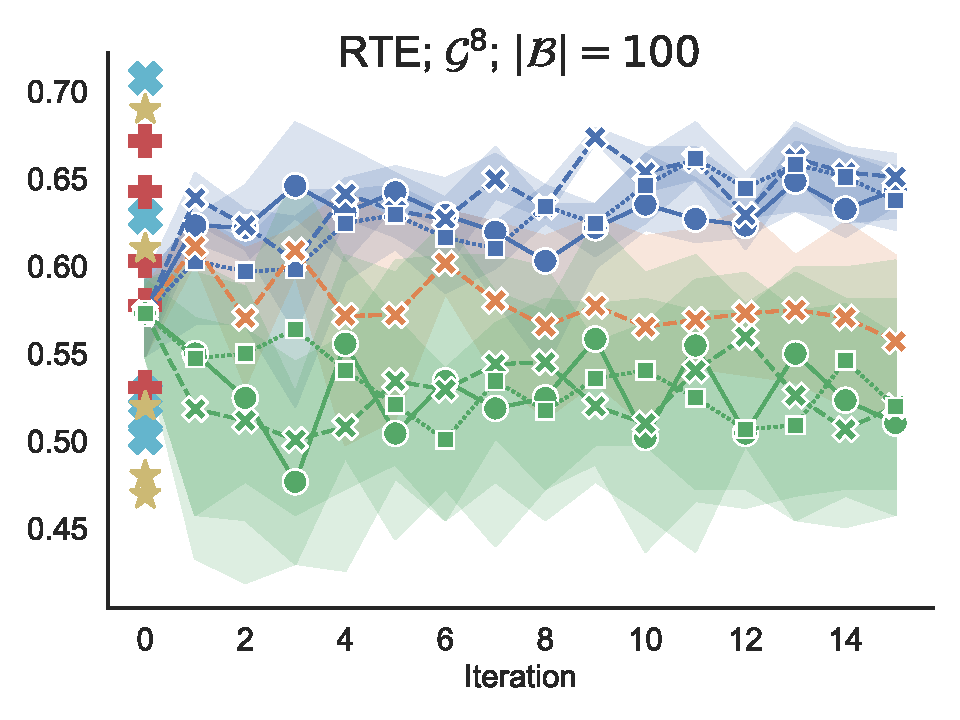
\includegraphics[width=.25\linewidth,height=0.2\textwidth]{imgs/appendix/_rte,MV,8,100.pdf}
}
\hspace{-.2cm}\subfloat{
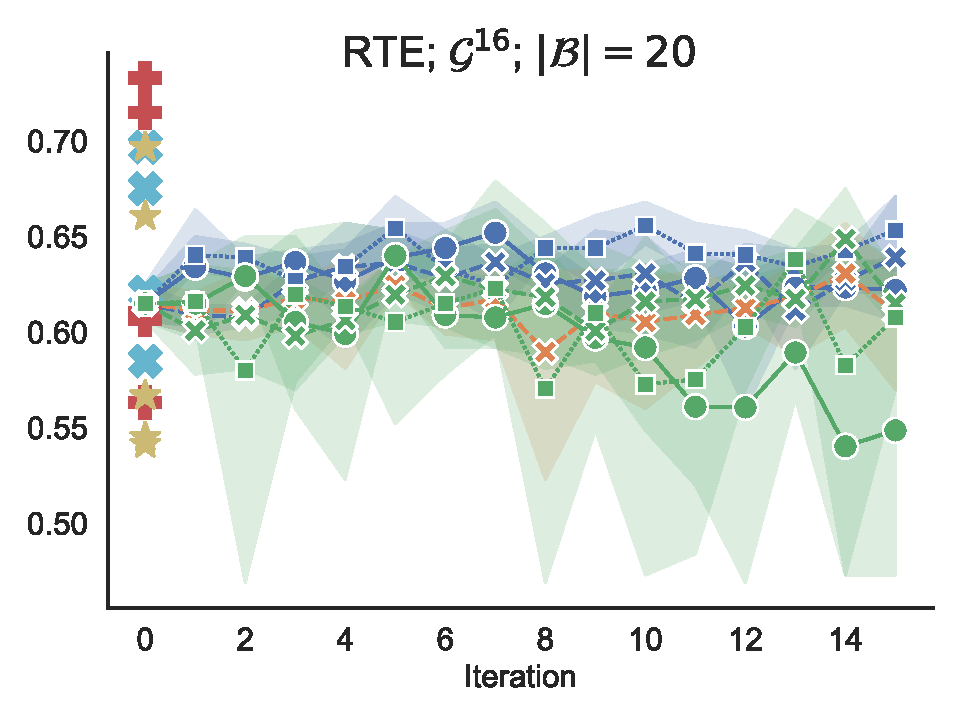
\includegraphics[width=.25\linewidth,height=0.2\textwidth]{imgs/appendix/_rte,MV,16,20.pdf}
}
\hspace{-.2cm}\subfloat{
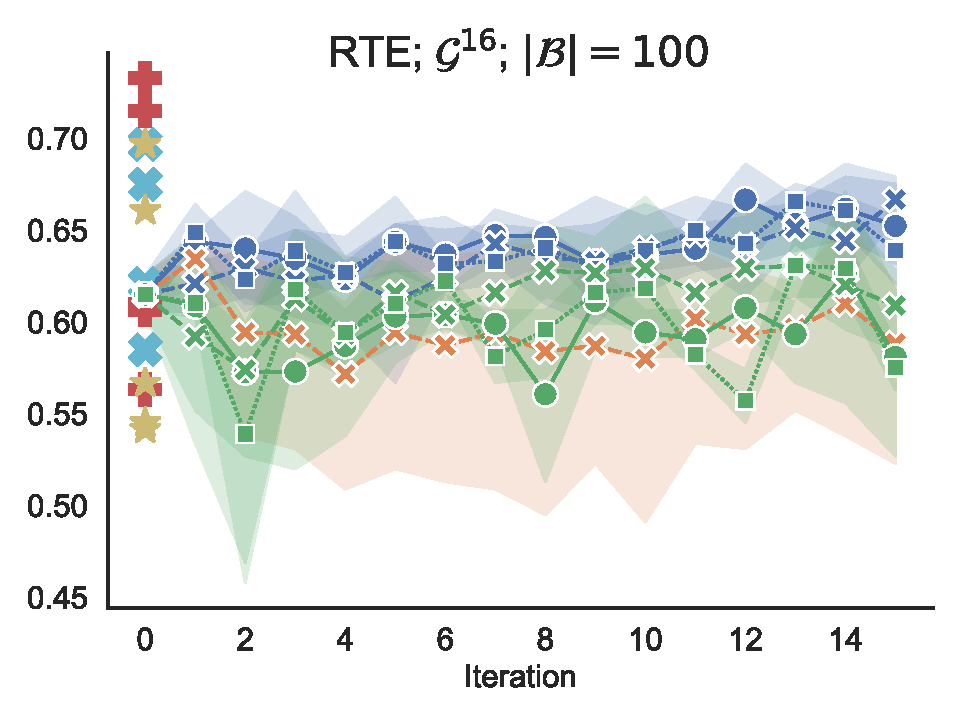
\includegraphics[width=.25\linewidth,height=0.2\textwidth]{imgs/appendix/_rte,MV,16,100.pdf}
}
\hspace{-.2cm}\subfloat{
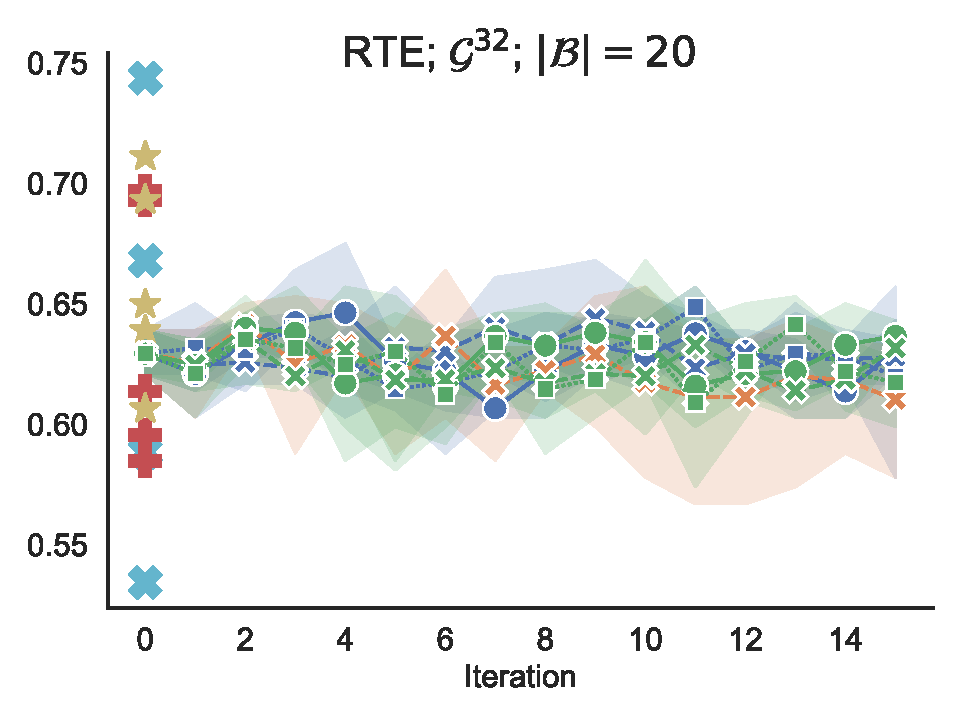
\includegraphics[width=.25\linewidth,height=0.2\textwidth]{imgs/appendix/_rte,MV,32,20.pdf}
}

\caption{
  Improving $\mathcal{S}$ with
  \textcolor{blue}{active learning (blue)},
  \textcolor{orange}{self training (orange)},
  and
  \textcolor{green}{\md (green)}.
  Free markers at step zero show \mdr performances;
  colors distinguish random seeds.
  Three acquisition functions are:
  Entropy ($\bullet$),
  LeastConfident (\tiny$\blacksquare$\normalsize),
  random sampling (\tiny\XSolidBold\normalsize).
  At iteration $j$, each experiment is repeated
  three times; we show
  mean and standard deviation.
  We evaluate different $|\mathcal{G}|$ and $|\mathcal{B}|$.
}
\figlabel{appendix:completeiteratives}
\end{figure*}




\section{Instance Weighting}
\seclabel{appendix:instanceweighting}
Following \citet{wang-etal-2017-instance},
we associate each example
$(\textbf{x}, \hat{y}, \textbf{l}) \in \mathcal{D}^{j}$
with weight
1-$entropy(\textbf{l})$ when
computing the loss during
training $\mathcal{S}^{j}$.
We can interpret this weight as a measure
of the certainty of the \mdrs ensemble.


\figref{instanceweighting} reports
the performance of $\mathcal{S}$
when using instance weighting,
however, the impacts are less noticeable.





%%% Local Variables:
%%% mode: latex
%%% TeX-master: "acl_latex"
%%% End:
